% Illustration of audio playback via loudspeakers

%*****************************************************************************
% Copyright (c) 2013-2019 Fiete Winter                                       *
%                         Institut fuer Nachrichtentechnik                   *
%                         Universitaet Rostock                               *
%                         Richard-Wagner-Strasse 31, 18119 Rostock, Germany  *
%                                                                            *
% This file is part of the supplementary material for Fiete Winter's         *
% scientific work and publications                                           *
%                                                                            *
% You can redistribute the material and/or modify it  under the terms of the *
% GNU  General  Public  License as published by the Free Software Foundation *
% , either version 3 of the License,  or (at your option) any later version. *
%                                                                            *
% This Material is distributed in the hope that it will be useful, but       *
% WITHOUT ANY WARRANTY; without even the implied warranty of MERCHANTABILITY *
% or FITNESS FOR A PARTICULAR PURPOSE.                                       *
% See the GNU General Public License for more details.                       *
%                                                                            *
% You should  have received a copy of the GNU General Public License along   *
% with this program. If not, see <http://www.gnu.org/licenses/>.             *
%                                                                            *
% http://github.com/fietew/publications           fiete.winter@uni-rostock.de*
%*****************************************************************************

\documentclass[beamer, tikz, ignorerest, crop]{standalone}

\usefonttheme{int}
\usecolortheme{int}

\usepackage{soundfield}

%% Color
\usepackage{color}
\definecolor{activecolor}{RGB}{150, 150, 150}
\definecolor{area}{RGB}{236, 236, 236}
\definecolor{local}{RGB}{254, 204, 0}

%% TikZ
\usetikzlibrary{calc,%
  decorations.pathreplacing,%
  decorations.markings,%
  calc,%
  angles,%
  arrows,%
  arrows.meta,%
  through,%
  intersections,%
  positioning,%
  shapes.callouts}
\usepackage{../audioicons}

% loudspeaker
\tikzstyle{loudspeaker} = [
basic loudspeaker, 
draw=black!70, 
fill=white, 
minimum height=3pt,
minimum width=1.5pt,
inner sep=0.5pt,
relative cone width=1.5,
relative cone height=2.5
]

% microphone
\tikzstyle{microphone} = [
  basic microphone,
  draw, 
  fill=gray!20, 
  membrane style=very thick,
  minimum width=8pt, 
  minimum height=8pt,
  inner sep=1pt
]

\tikzset{
  mark coordinate/.style args={(#1) at #2}{
    postaction={
      decorate,
      decoration={
        markings,
        mark=at position #2 with {\coordinate (#1);}
      }
    }
  }
}

\tikzset{
  mark node/.style args={(#1) at #2 with #3}{
    postaction={
      decorate,
      decoration={
        markings,
        mark=at position #2 with {\node[#3](#1) {};}
      }
    }
  }
}

\tikzset{
  add loudspeakers/.style args={#1}{
    postaction={
      decorate,
      decoration={
        markings,
        mark=between positions 0 and 1 step 1/#1 with {%
          \node[loudspeaker,
          fill=activecolor,
          transform shape,
          rotate=90,
          anchor=cone] {};
        },
      }
    }
  }
}

\tikzstyle{superblock} = [fill=black!10, draw, very thick, rounded corners]
\tikzstyle{block}[5.5cm] = [minimum height= 4cm, minimum width=#1, draw, very 
thick, fill=white]
\tikzstyle{both}[5.5cm] = [block=#1, fill=green!20]
\tikzstyle{matlab}[5.5cm] = [block=#1, fill=red!20]
\tikzstyle{python}[5.5cm] = [block=#1, fill=blue!20]
\tikzstyle{planned}[5.5cm] = [block=#1, dashed]
\tikzset{>={Stealth[inset=0pt,length=0.5cm,angle'=28,round]}}
\tikzstyle{connect} = [draw=black, very thick, ->]
\tikzstyle{exchange} = [draw=black, very thick, <->]


\begin{document}
\begin{tikzpicture}
  
%\path[draw=black!80, thick, fill=black!20] (-3.7,-1.8) rectangle(3.7,4.2);

% \useasboundingbox (-3.7,-1.8) rectangle(3.7,4.2);

%\path[draw=black!80, thick, fill=red!10] (-3.5,-1.6) rectangle(3.5,4.0);

\pgfmathsetmacro{\xRecOne}{-1.5}
\pgfmathsetmacro{\yRecOne}{0.5}
\pgfmathsetmacro{\rMicarray}{0.5}
\pgfmathsetmacro{\xMicarray}{-0.75}
\pgfmathsetmacro{\yMicarray}{1.7}

\pgfmathsetmacro{\xRecTwo}{-1.5}
\pgfmathsetmacro{\yRecTwo}{-3.5}
\pgfmathsetmacro{\xMic}{-0.5}
\pgfmathsetmacro{\yMic}{+1.2}

\pgfmathsetmacro{\xLis}{1.5}
\pgfmathsetmacro{\yLis}{-3.5}

\pgfmathsetmacro{\xHead}{2.0}
\pgfmathsetmacro{\yHead}{3.5}

\pgfmathsetmacro{\rLs}{2.65}
\pgfmathsetmacro{\phiLs}{40}

\pgfmathsetmacro{\phiWaves}{45}

\node[rectangle, draw, minimum height=1cm] (dsp) {Signalverarbeitung};

% additional anchors for dsp
\foreach \direction in {north, south}{
  \foreach \rdx in {1, 2, ..., 9}{
    
    \pgfmathsetmacro{\ratio}{1-\rdx/10}
    \pgfmathsetmacro{\ratioInv}{1-\ratio}
    \edef\west{ west}
    \edef\east{ east}
    \coordinate (dsp\direction\rdx) 
      at ($\ratio*(dsp.\direction  \west) + \ratioInv*(dsp.\direction  \east)$);
  }
}

% first recording environment
\begin{scope}[shift={(\xRecOne,\yRecOne)}]

  \node[anchor=north east] {Aufnahmeumgebungen};

  \draw[very thick] (0,0) rectangle (-2*\xHead,2.5);

  \coordinate (miccenter) at (\xMicarray,\yMicarray);
  
  \foreach \phi in {45, 90, ..., 315} {  
    \node[microphone, fill=activecolor, rotate=180+\phi, 
    scale=0.75] 
      (micarray\phi) at ($(miccenter)+(\phi:\rMicarray)$) {};
    \draw (miccenter) -- (micarray\phi);
  }

  \node[inner sep=0pt] at ($(miccenter)+(-1.9,-0.7)$)
    {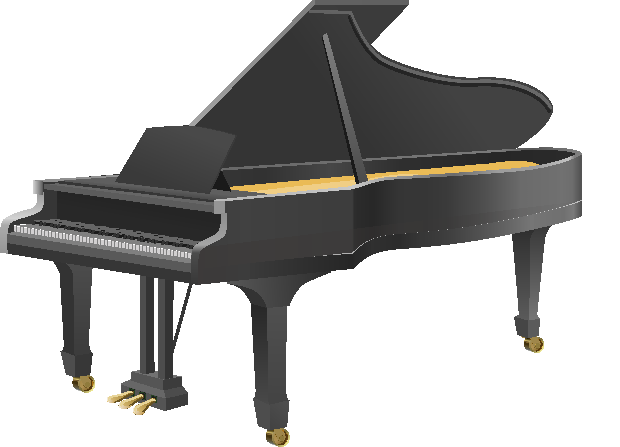
\includegraphics[width=2.5cm]{piano.pdf}};
\end{scope}
\draw[-latex', thick] (miccenter) -| (dspnorth2);

% second recording environment
\begin{scope}[shift={(\xRecTwo,\yRecTwo)}]
  %
  \draw[very thick] (0,0) rectangle +(-2*\xHead,3.5);
  % microphones
  \foreach \idx/\ratio in {1/0,2/1} {%
    \node[microphone, anchor=west, fill=activecolor,scale=0.75] 
      (mic\idx) at (\xMic-\ratio*1,\yMic+\ratio*1.3) {};
  }%
  
  \node[left=-0.2cm of mic2, inner sep=0pt] 
    {\rotatebox{-45}{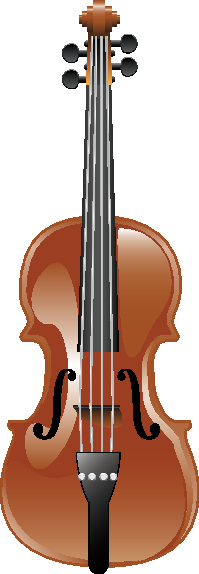
\includegraphics[width=0.65cm]{violin.pdf}}};
  \node[left=-0.2cm of mic1, inner sep=0pt]  
    {\rotatebox{-45}{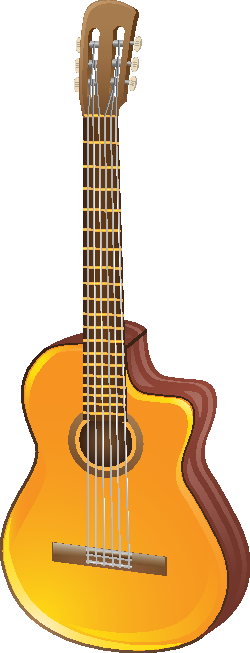
\includegraphics[width=1.0cm]{guitar.pdf}}};
\end{scope}

\draw[-latex'] (mic1) -| (dspsouth3) node[pos=0.8,right]{Audiosignale};
\draw[-latex'] (mic2) -| (dspsouth2);

% listening environment
\begin{scope}[shift={(\xLis,\yLis)}]

  \node[anchor=north west,inner sep=0] at (0,-0.1) {Wiedergabeumgebung};

  \draw[very thick] (0,0) rectangle +(2*\xHead,6.0);
  
  \node[rotate=90] (head) at (\xHead,\yHead)  
    {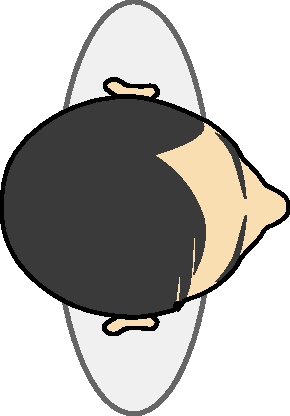
\includegraphics[scale=0.2]{head.pdf}}; 
    
  \node[cloud callout,%
    cloud puff arc=110,%
    cloud puffs=14,%
    callout pointer width=1,%
    callout absolute pointer={(head.west)},%
    callout pointer segments=2,%
    aspect=2.0,%
    fill=black!20,% 
    below,%
    draw=black!40,
    thick,%
    minimum width=3.8cm,%
    minimum height=2cm] (cloud) at ($(head)+(0,-1.25)$) {};
  
  \node[inner sep=0pt] at ($(cloud)+(-0.8,0.2)$)
    {\rotatebox{-45}{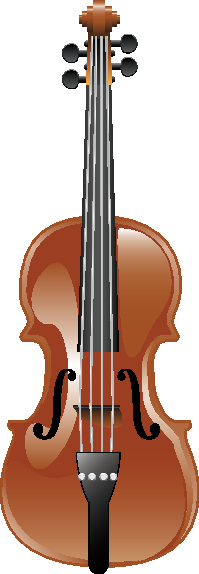
\includegraphics[width=0.45cm]{violin.pdf}}};
  \node[inner sep=0pt] at ($(cloud)+(-0.1,0)$)
    {\rotatebox{-45}{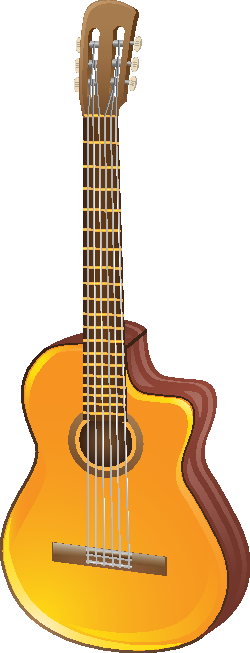
\includegraphics[width=0.6cm]{guitar.pdf}}};
  \node[inner sep=0pt] at ($(cloud)+(0.9,0)$)
    {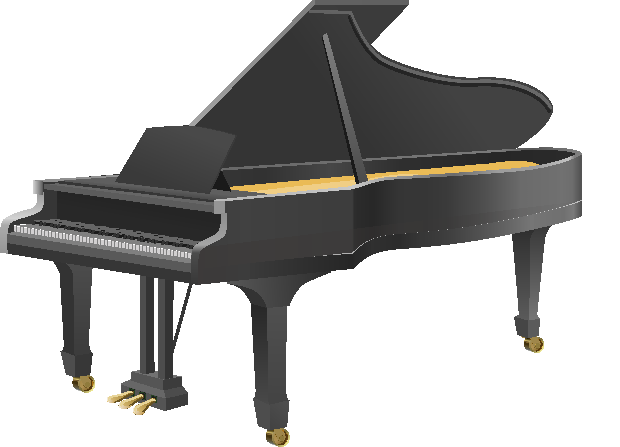
\includegraphics[width=1.5cm]{piano.pdf}};
    
  \foreach \idx/\phi in {1/-\phiLs, 2/\phiLs} {    
    % loudspeakers
    \node[loudspeaker, anchor=cone, scale=1.5, fill=activecolor, 
      rotate=\phi-90] (ls\idx) at ($(head)+(90+\phi:\rLs)$) {};
    
    % sound waves
    \foreach \Rwaves in {0.3, 0.5, 0.7}{
      \draw[draw=black] ($(ls\idx.cone)+(90+\phi+\phiWaves:-\Rwaves)$) arc 
        (90+\phi+\phiWaves:90+\phi-\phiWaves:-\Rwaves);
    }
  }
\end{scope}

\draw[latex'-] (ls1) |- +(0,0.8) -| (dspnorth8) ;
\draw[latex'-] (ls2) |- +(0,0.6) -| (dspnorth9) ;

\end{tikzpicture}
\end{document}
